
\section{Архитектура и модули системы} % (fold)
\label{sec:arch_and_mod}

Разработанное программное средство представляет из себя клиент-серверное приложение, в котором клиентом выступает браузер, а сервером — веб-сервер. Логика веб-приложения распределена между сервером и клиентом, хранение данных осуществляется, преимущественно, на сервере, обмен информацией происходит по сети. Одним из преимуществ такого подхода является тот факт, что клиенты не зависят от конкретной операционной системы пользователя. Исходя из выше сказанного, можно сказать, что веб-приложения являются кроссплатформенными сервисами. Серверная часть приложения реализована с помощью языка Java. Клиентская часть реализована с помощью языка Javascript.

Серверная часть состоит из следующих модулей:
\begin{itemize}
	\item модуль доступа к данным (DAO);
	\item модуль сервисов(Бизнес логика);
	\item модуль предоставления данных(Форматирование данных);
\end{itemize}

Клиентская часть состоит из следующих компонентов:
\begin{itemize}
	\item модуль действий(actions);
	\item модуль отображений(components);
\end{itemize}

Рассмотрим каждый компонент по отдельности. 

\subsection{Модуль доступа к данным}
\label{sub:arch_and_mod:lexer}

Данный модуль дает возможность доступа к базе данных. Для реализации данной функциональности использовался шаблон проектирования DAO. 

Шаблон проектирования DAO -- это объект, который предоставляет абстрактный интерфейс к какому-либо типу базы данных или механизму хранения. Определённые возможности предоставляются независимо от того, какой механизм хранения используется и без необходимости специальным образом соответствовать этому механизму хранения. Этот шаблон проектирования применим ко множеству языков программирования, большинству программного обеспечения, нуждающемуся в хранении информации и к большей части баз данных. На данном  уровне нет механизма для управления транзакциями, т.к. транзакции как правило принимают участие в бизнес операциях.  

В качестве выбора данного шаблона, послужили следующие факторы:

\begin{itemize}
	\item DAO инкапсулирует доступ к источнику данных;
	\item DAO является реализацией слоя объектно-реляционного отображения;
	\item DAO более ориентирован на источник данных;
\end{itemize}


Основная цель данного модуля --- упростить процесс взаимодействия с БД. Пример реализации шаблона DAO приведены в листинге~\ref{lst:arch_and_mod:DAO}:

\begin{lstlisting}[language=Java, style=rubystyle, caption={Определение для доступа к данным}, label=lst:arch_and_mod:DAO]
public interface IDAO<Key extends Serializable, E> {

E create(E entity);

E read(Key key);

void update(E entity);

void delete(E entity);

}

public abstract class AbstractDAOImp<Key extends Serializable, E> implements IDAO<Key, E> {

@Autowired
private SessionFactory sessionFactory;

private Class<E> clazz;

protected AbstractDAOImp(Class<E> clazz) {
	this.clazz = clazz;
}

protected Session getSession() {
	return sessionFactory.getCurrentSession();
}

@Override
public E create(E entity) {
	Session session = getSession();
	session.persist(entity);
	session.flush();
	return entity;
}

@Override
public E read(Key key) {
	return getSession().find(clazz, key);
}

@Override
public void update(E entity) {
	getSession().update(entity);
}

@Override
public void delete(E entity) {
	getSession().delete(entity);
}

}

@Repository("UserRepository")
public class UserDAOImp extends AbstractDAOImp<Integer, User> {

protected UserDAOImp() {
	super(User.class);
}

public List<User> readAllUser() {
	return getSession().createQuery("from users", User.class).list();
}

}
\end{lstlisting}


\subsection{Модуль сервисов}~
\label{sec:arch_and_mod:regex}
На этом уровне реализована бизнес логика приложения, управление транзакциями, сервис для загрузки изображений и другие. 

Для начала рассмотрим сервис, который взаимодействует с модулем DAO. Сервис для взаимодейсвтия с DAO приведен в листинге~\ref{lst:arch_and_mod:Service1}:

\begin{lstlisting}[language=Java, style=rubystyle, caption={Использование DAO в сервисах}, label=lst:arch_and_mod:Service1]

@Service("UserService")
@Transactional
public class UserService {

@Autowired
private UserDAOImp daoImp;

public User addUser(User user) {
	return daoImp.create(user);
}

public void updateUser(User user) {
	daoImp.update(user);
}

public void removeUser(User user) {
	daoImp.delete(user);
}

public List<User> findAllUser() {
	return daoImp.readAllUser();
}

public User findUserById(int id) {
	return daoImp.read(id);
}

}

@Service("CommentService")
@Transactional
public class CommentService {

@Autowired
private CommentDAOImp daoImp;

public Post addPost(Comment comment){
return daoImp.create(comment);
}

public Post findCommentById(int id){
return daoImp.read(id);
}

public void updateComment(Post post){
daoImp.update(post);
}

public void removeComment(Post post){
daoImp.delete(post);
}

}

\end{lstlisting}

Сначала может показаться, что модуль сервис повторяет методы класса DAO. Но эти методы не просто повторяют, они оборачивают методы DAO с использованием транзакций. Транзакция это группа последовательных операций с базой данных, которая представляет собой логическую единицу работы с данными. Транзакция может быть выполнена либо целиком и успешно, соблюдая целостность данных и независимо от параллельно идущих других транзакций, либо не выполнена вообще, и тогда она не должна произвести никакого эффекта. Можно заметить, что модуль сервисов зависит от модуля DAO.

Рассмотрим сервис для загрузки и сохранения изображений. При разработке приложений была обнаружена проблема с быстрой загрузкой графического контента. Если картинки довольно большие, то необходимо обеспечить эффективную работу с памятью для предотвращения злополучной ошибки OutOfMemoryError. Так же во время загрузки изображения было необходимо показывать маленькое изображение. Именно данная проблематика и подталкивает обратиться к библиотеке с открытым исходным кодом – Universal Image Loader, целью которой является универсализация решения вышеописанной задачи в виде гибкого и конфигурируемого инструмента.

На данный момент библиотеку можно использовать в тех случаях, когда нужно загрузить и отобразить (и можно еще закэшировать) картинку из интернета или из файловой системы. Классические примеры применения ImageLoader'а – это списки, таблицы, галереи, где необходимо отображать изображения из сети.

Среди возможностей ImageLoader'а можно выделить следующие до-стоинства:

\begin{itemize}
	\item асинхронная загрузка и отображение изображений из интернета или с SD-карты;
	\item возможность кэширования загруженных картинок в памяти и/или на файловой системе устройства;
	\item возможность отслеживания процесса загрузки посредством «слушателей»;
	\item эффективная работа с памятью при кэшировании картинок в памяти;
	\item широкие возможности настройки ImageLoader'а.
\end{itemize}

К глобальным настройкам ImageLoader'а можно отнести:

\begin{itemize}
	\item максимальный размер кэшируемых в памяти картинок;
	\item тайм-аут для установки соединения и загрузки картинки;
	\item максимальное количество потоков для загрузки изображений, работающих одновременно;
	\item приоритет потоков по загрузке и отображению картинок;
	\item программная реализация дискового кэша (можно выбрать одну из готовых реализаций или создать свою собственную);
	\item программная реализация кэша в памяти (можно выбрать одну из готовых реализаций или создать свою собственную);
	\item опции загрузки изображения по умолчанию.
\end{itemize}

Опции загрузки изображения (применяются к каждому отдельному вызову ImageLoader.displayImage(...)) предоставляют возможность указать:

\begin{itemize}	
	\item отображать ли картинку – заглушку в ImageView, пока реальная картинка грузится (если да, то нужно указать эту «заглушку»);
	\item отображать ли какую-либо картинку в ImageView, если URL кар-тинки был передан пустым (если да, то нужно указать эту картинку); 
	\item кэшировать ли загруженную картинку в памяти;
	\item кэшировать ли загруженную картинку на файловой системе;
	\item тип декодирования изображения (максимально быстрый или мак-симально экономный для памяти).
\end{itemize}


\begin{figure}[!htb]
			\centering
			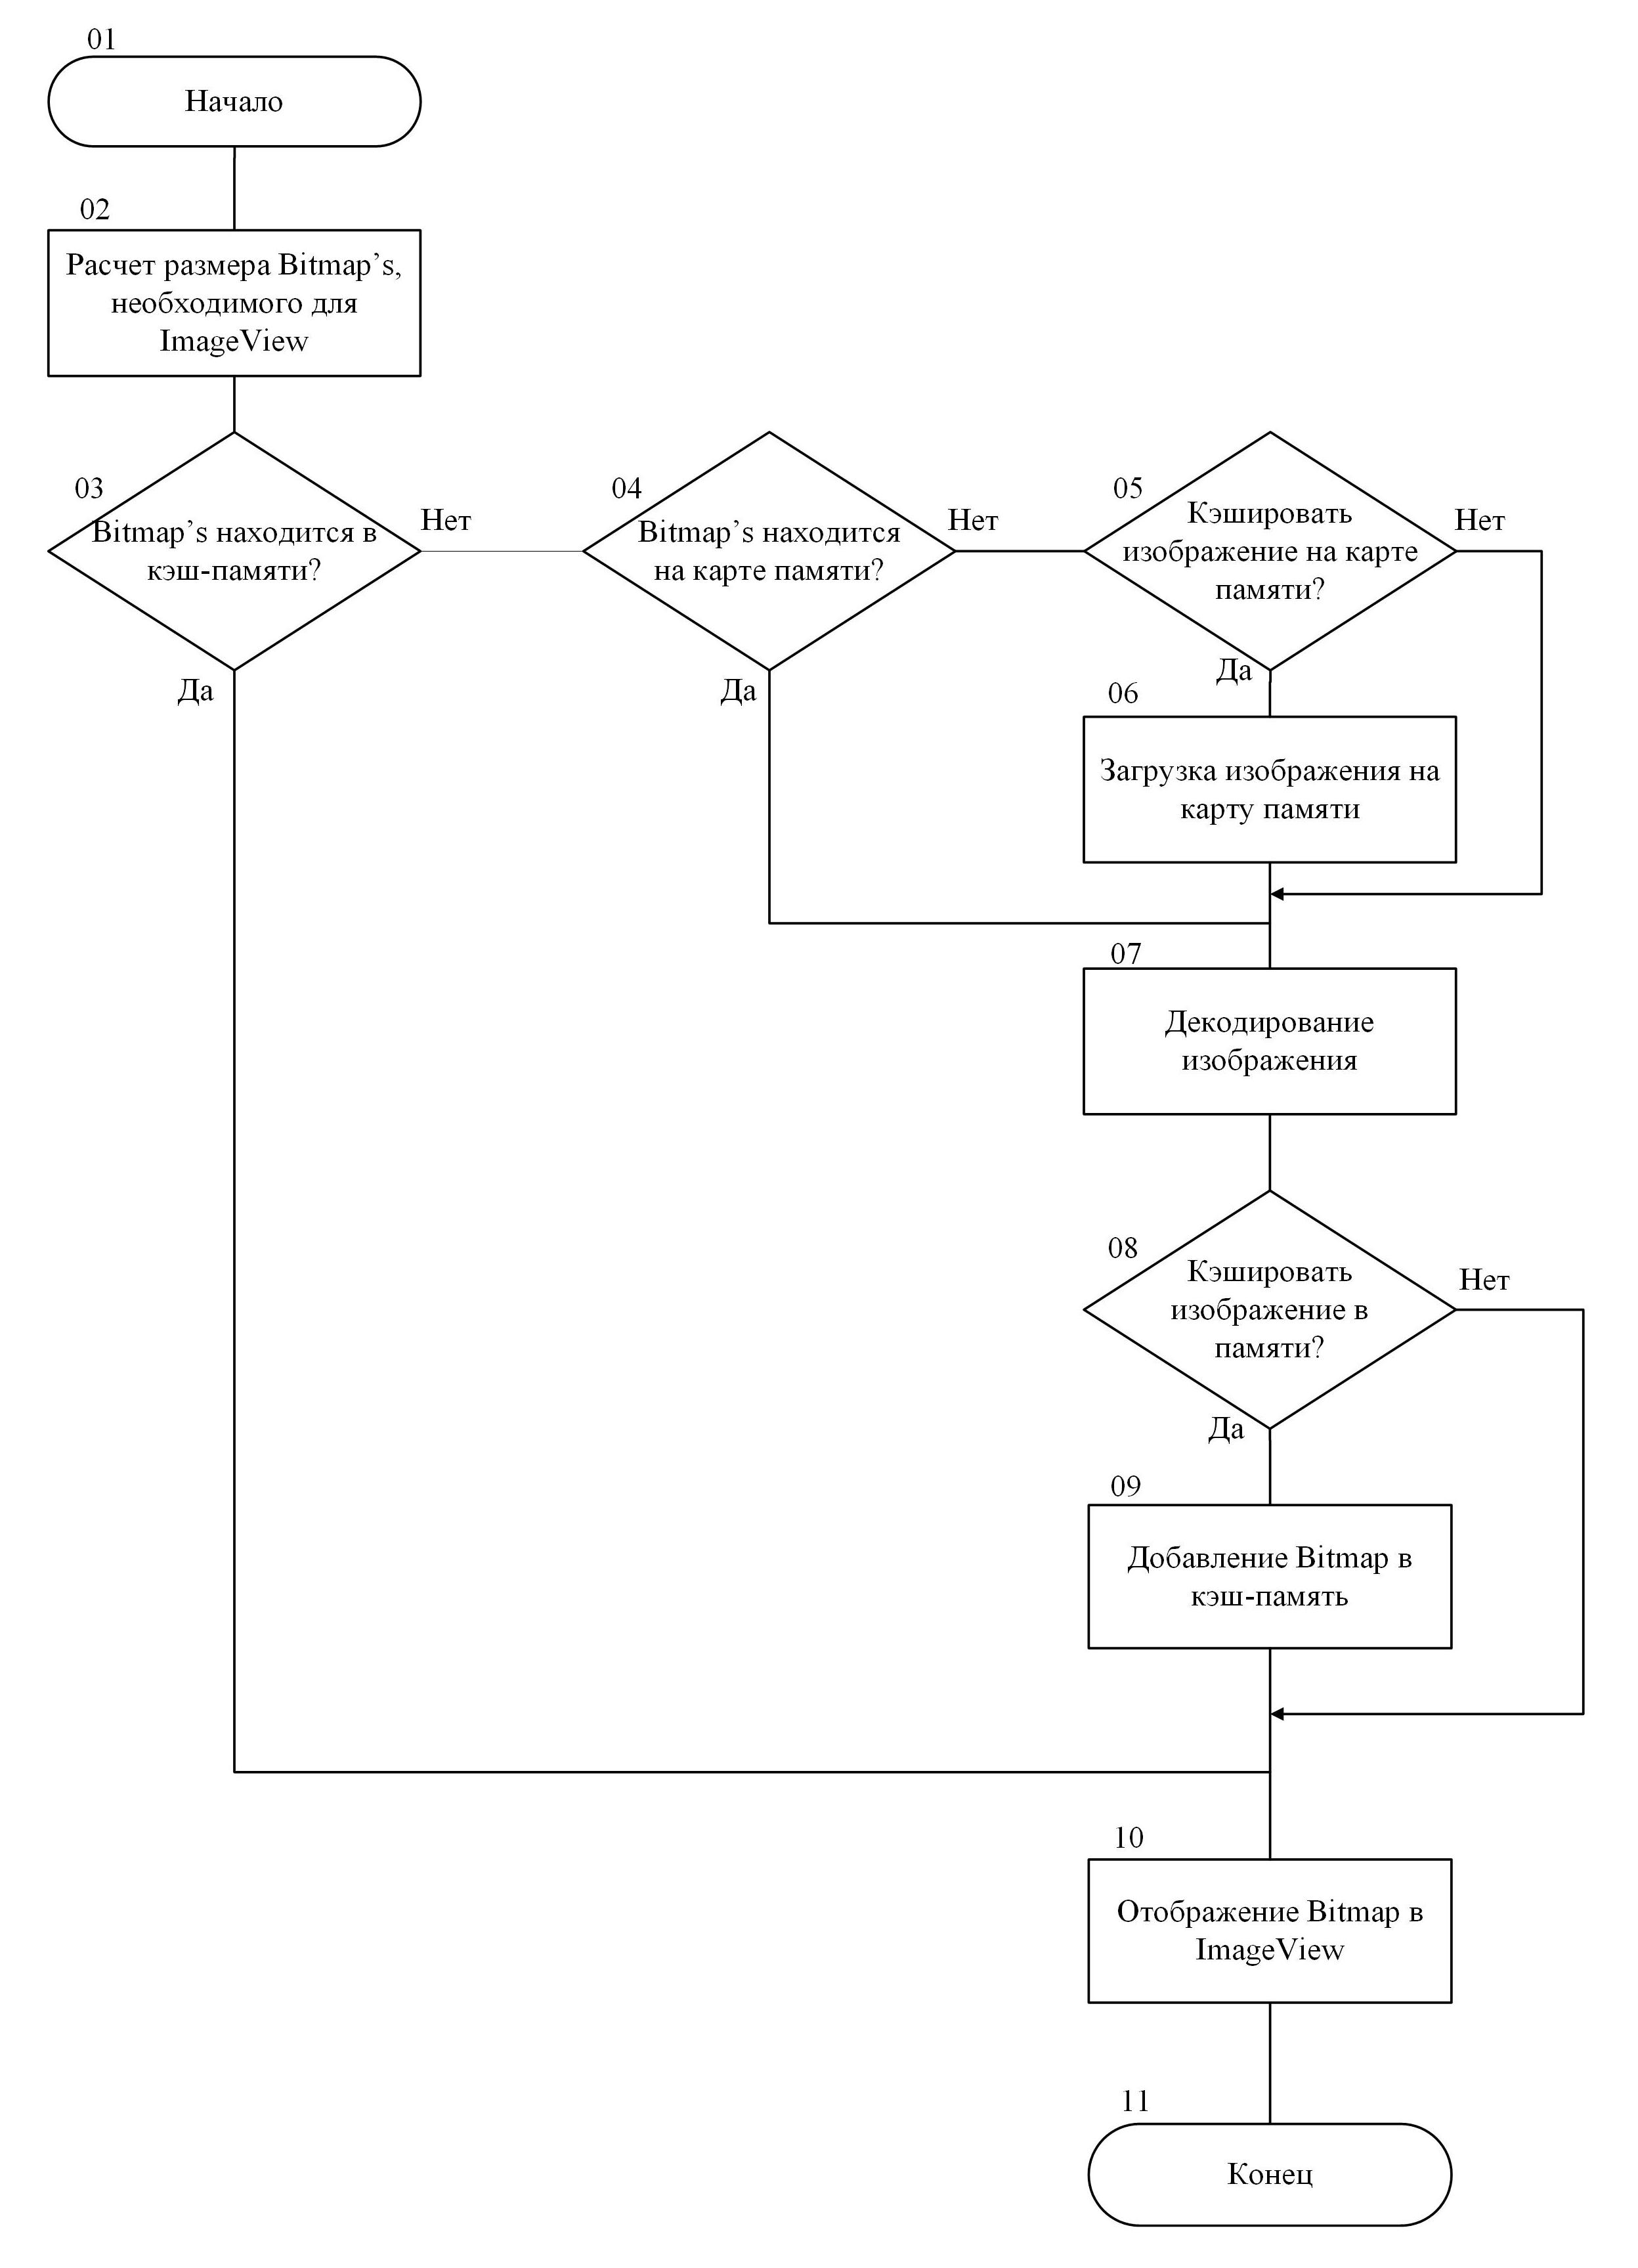
\includegraphics[scale=0.28]{loadImage.jpg}
			\caption{ Схема алгоритма ImageLoader }
			\label{fig:arch_and_mod:ImageLoader}
\end{figure}

Как уже упоминалось, программные реализации дискового кэша и кэша в памяти можно подключить свои. Но, скорее всего, будет достаточ-но готовых решений, которые в большинстве своем представляют собой кэши, ограниченные по какому-либо параметру (размер, количество файлов) и имеющие свою логику самоочищения при превышении лимита (FIFO, самый старый объект, самый большой объект, наиболее редко используемый).


Каждая задача на загрузку и отображение картинки выполняется в отдельном потоке, кроме случаев, если картинка находится в кэше в памяти. Тогда она просто сразу отображается. Существует отдельная очередь потоков, куда попадают задачи, если нужная картинка закэширована на файловой системе. 

Если же нужной картинки нет в кэше, то задача-поток попадает в пул пото-ков. Таким образом, быстрому отображению закэшированных картинок ничего не препятствует.

Для управления загрузкой картинок, используется класс ImageLoaderService. Это singletone, поэтому чтобы получить единственный экземпляр класса нужно вызвать метод getInstance(). Перед использованием ImageLoader'а по назна-чению (для отображения картинок), необходимо проинициализировать его конфигурацией.

Самый простой вариант использования ImageLoader'a (с конфигурацией по умолчанию) представлен  в листинге~\ref{lst:arch_and_mod:Service2}:

\begin{lstlisting}[language=Java, style=rubystyle, caption={Определение ImageLoaderService}, label=lst:arch_and_mod:Service2]
@PropertySource(value = { "classpath:imageLoader.properties" })
@Service("ImageLoaderService")
public class ImageLoaderService {

@Autowired
private Environment environment;
private static ImageLoader imageLoader;

public ImageLoader getInstance() {
if(imageLoader == null){
ImageLoader imageLoader = ImageLoader.init(getProperties());
}
return imageLoader;
}


private Properties getProperties() {
Properties properties = environment.loadConfiguration();
return properties;
}

}
\end{lstlisting}


\subsection{Модуль предоставления данных}
\label{sub:arch_and_mod:parser}
Следующий за модулем сервисов --- модуль предоставляения данных. Для обработки клиентских запросов используются \textit{spring controllers}.
 
Spring controllers --- это классы, которые осуществляют обработку запроса от клиента (браузера). Здесь происходит валидация данных, передача данных в модуль сервисы. Завершающим этапом будет генерация и форматирование ответа в формат \textit{JSON}.

JSON --- это текстовый формат обмена данными, основанный на JavaScript. Как и многие другие текстовые форматы, JSON легко читается. За счёт своей лаконичности по сравнению с XML, формат JSON был более подходящим для сериализации сложных структур. Если говорить о веб-приложениях, формат уместен в задачах обмена данными между браузером и сервером.

Бизнес логика приложения в этом модуле не присутствует, она делегируется модулю сервисов.

В качестве примера рассмотрим controller, который отвечает за регистрацию и входа пользователя в систему. Класс LoginController представлен в листинге~\ref{lst:arch_and_mod:Service3}:

\begin{lstlisting}[language=Java, style=rubystyle, caption={Определение LoginController}, label=lst:arch_and_mod:Service3]
@Controller
@RequestMapping(value="api/user"
public class LoginController{

@Autowired
private LoginService loginService;

@Autowired
private UserService userService;

@RequestMapping(value="/signin",method=RequestMethod.GET)
public String signIn(HttpServletRequest request, HttpServletResponse response){
String username = request.getParameter("login");
String password = request.getParameter("password");

boolean isValidUser = loginService.isValidUser(username, password);
User user = null;
if(isValidUser){
user = userService.findUserByLogin(username, password);
}

return ObjectMapper.toJSON(user);
}


@RequestMapping(value="/signup",method=RequestMethod.POST)
public HttpServletResponse signUp(HttpServletRequest request, HttpServletResponse response) {
String username = request.getParameter("login");
String password = request.getParameter("password");

boolean isValidUser = loginService.isValidUser(username, password);
if(isValidUser){
userService.createUser(username, password)
response.setAttribute("signUp", "Success operation. You will be redirected to sign in page!");
}else{ 
response.setAttribute("signUp", "Invalid operation. Please, specify correct usernamge, email!");
}
return response;
}

}
\end{lstlisting}

Метод signIn нужен для входа в программное средство. Данный метод включает в себя запрос от клиента и будущий ответ. Для начала входа систему, необходимо получить имя пользователя и его пароль. Если такой пользователь существует, то система загружает пользователя и формирует ответ на клиент. Строка \textit{ObjectMapper.toJSON} преобразует джава объект в формат JSON. Этот ответ будет обработан клиентом. 

Метод signUp нужен для регистрации пользователя в программном средстве.  Данный метод включает в себя запрос от клиента и будущий ответ. Для регистрации в программном средстве, необходимо получить имя пользователя и  пароль, который прислал клиент в запросе. Далее проверяется, если такой пользователь не существует в системе, то пользователь будет создан, иначе происходит уведомление клиента о некорректности передаваемых данных.


\subsection{Модуль действий}
Рассмотрим модуль действий. Модуль находиться на клиентской части и отвечает за взаимодействие со слоем предоставления данных. Данный модуль общается посредством \textit{http} и \textit{ajax}. 

HTTP — широко распространённый протокол передачи данных, изначально предназначенный для передачи гипертекстовых документов (то есть документов, которые могут содержать ссылки, позволяющие организовать переход к другим документам). Http метод представляет собой последовательность из любых символов, кроме управляющих и разделителей, и определяет операцию, которую нужно осуществить с указанным ресурсом. 

AJAX --- подход к построению интерактивных пользовательских интерфейсов веб-приложений, заключающийся в «фоновом» обмене данными браузера с веб-сервером. В результате, при обновлении данных веб-страница не перезагружается полностью, и веб-приложения становятся быстрее и удобнее. AJAX — не самостоятельная технология, а концепция использования нескольких смежных технологий. 
AJAX базируется на двух основных принципах:

\begin{itemize}
	\item использование технологии динамического обращения к серверу «на лету», без перезагрузки всей страницы полностью, например с использованием XMLHttpRequest (основной объект);
	\item использование DHTML для динамического изменения содержания страницы;
\end{itemize}

В качестве формата для обмена данных между клиентом и сервером используется JSON.

Первый пример демонструет вход в систему. LoginAction представлен в листинге~\ref{lst:arch_and_mod:Service4}:

\begin{lstlisting}[language=Java, style=rubystyle, caption={Определение LoginAction}, label=lst:arch_and_mod:Service4]

var LoginAction = {

signIn: function(nickname, password, callback){

	$.ajaxPost("/api/user/signIn", {"nickname": nickname, "password": password}, function (data) {
		callback(data);
	});

}

}
\end{lstlisting}

Рассмотри ситуацию, когда пользователь хочет оставить комментарий на недвижимость. Пользователь может добавить комментарий, удалить комментарий, редактировать комментарий, читать предыдущие комментарии. В рамках этих условий, был разработан модуль CommentsActions, который выполняет все вышеперечисленные действия. CommentsActions представлен в листинге~\ref{lst:arch_and_mod:Service5}:

\begin{lstlisting}[language=Java, style=rubystyle, caption={Определение CommentsActions}, label=lst:arch_and_mod:Service5]
var CommentsActions = {

addComment: function(text, callback){
	$.ajaxPost("/api/comments/addComment/", function (data) {
		if (callback) {
			callback(data);
		}       
	});
},

removeComment: function(id, callback){
	$.ajaxPost("/api/comments/removeComment/", {"id":id}, function (data) {
		if (callback) {
			callback(data);
		}
	});
},

editComment: function(id, text, callback){
	$.ajaxPost("/api/comments/editComment/", {"id":id, "text":text}, function (data) {
		if (callback) {
			callback(data);
		}
	});
},

loadAllComments:function(id, callback){
	$.ajaxPost("/api/comments/loadAll/", {"id":id}, function (data) {
		if (callback) {
		callback(data);
		}
	});
}

}

\end{lstlisting}

Подобным обазом работают и другие функции. Сначала указываться url для запроса на сервер. Далее перечесляются обязательные параметры для сервиса. Следующим параметрам идет функцию в которую придет ответа от севера. Если ответ удволетворяет условию, будет вызвана \textit{callback функция}.

Callback функция или функция обратного вызова в программировании — передача исполняемого кода в качестве одного из параметров другого кода. Обратный вызов позволяет в функции исполнять код, который задаётся в аргументах при её вызове. 

В момент, когда ответит ajax запрос, будет вызва функция обратного вызова. Обработка ответа будет представлена в месте, где используется модуль действия. 

\subsection{Модуль отображения}

Рассмотрим модуль отображений. Модуль находиться на клиентской части и отвечает за взаимодействие со слоем действий. Данный модуль непосредственно отображает информацию для конечного пользователя. 
Для реализации данного модуля, была выбрана библиотека \textit{React}. 

React --- уровень представления данных. React дает язык шаблонов и некоторые callback-функции для отрисовки HTML. Весь результат работы React --- это готовый HTML. Компоненты react занимаются тем, что хранят свое внутреннее состояние в памяти (например: какая закладка выбрана), но в итоге отображается html. 

Библиотека была выбрана из-за следующих плюсов:
\begin{itemize}
	\item Всегда можно сказать, как компонент будет отрисован, глядя на исходный код;
	\item Связывание JavaScript и HTML в JSX делает компоненты простыми для понимания;
	\item Можно генерировать html на сервере;
\end{itemize}

Рассмотрим форму для регистрации, реализованую с помощью библиотеки React. Код представлен в листинге~\ref{lst:arch_and_mod:Service6}:

\begin{lstlisting}[language=Java, style=rubystyle, caption={Форма регистрации LoginAction}, label=lst:arch_and_mod:Service6]

import React, { PropTypes } from 'react';
import { Link } from 'react-router';
import { Card, CardText } from 'material-ui/Card';
import RaisedButton from 'material-ui/RaisedButton';
import TextField from 'material-ui/TextField';


const LoginForm = ({
onSubmit,
onChange,
errors,
user
}) => (
<Card className="container">
<form action="/" onSubmit={onSubmit}>
<h2 className="card-heading">Login</h2>

{errors.summary && <p className="error-message">{errors.summary}</p>}

<div className="field-line">
<TextField
floatingLabelText="Email"
name="email"
errorText={errors.email}
onChange={onChange}
value={user.email}
/>
</div>

<div className="field-line">
<TextField
floatingLabelText="Password"
type="password"
name="password"
onChange={onChange}
errorText={errors.password}
value={user.password}
/>
</div>

<div className="button-line">
<RaisedButton type="submit" label="Log in" primary />
</div>

<CardText>Don't have an account? <Link to={'/signup'}>Create one</Link>.</CardText>
</form>
</Card>
);

LoginForm.propTypes = {
onSubmit: PropTypes.func.isRequired,
onChange: PropTypes.func.isRequired,
errors: PropTypes.object.isRequired,
user: PropTypes.object.isRequired
};

export default LoginForm;

import React, { PropTypes } from 'react';
import { Link, IndexLink } from 'react-router';


const Base = ({ children }) => (
<div>
<div className="top-bar">
<div className="top-bar-left">
<IndexLink to="/">React App</IndexLink>
</div>

<div className="top-bar-right">
<Link to="/login">Log in</Link>
<Link to="/signup">Sign up</Link>
</div>

</div>

{children}

</div>
);

Base.propTypes = {
children: PropTypes.object.isRequired
};

export default Base;

import Base from './components/Base.jsx';
import HomePage from './components/HomePage.jsx';
import LoginPage from './containers/LoginPage.jsx';
import SignUpPage from './containers/SignUpPage.jsx';


const routes = {
// base component (wrapper for the whole application).
component: Base,
childRoutes: [

{
path: '/',
component: HomePage
},

{
path: '/login',
component: LoginPage
},

{
path: '/signup',
component: SignUpPage
}

]
};

export default routes;
\end{lstlisting}

В React имеет компоненты, состояние, рендер. Компонент включает в себя html и функции для управления элементами на странице. Рендер предоставляет конечный вариант HTML браузеру (то, что видит пользователь). В некоторых компонентах нужно сохранять внутреннее состояние, которое используется во время визуализации. Например, флажок должен помнить, что он был выбран. Для этого используется функция состояние.

В завершении, рассмотрим диаграмму компонентов, отражающая работу всего приложения. Диаграмма представлена на рисунке \ref{fig:arch_and_mod::components}

\begin{figure}[!htb]
  \centering
  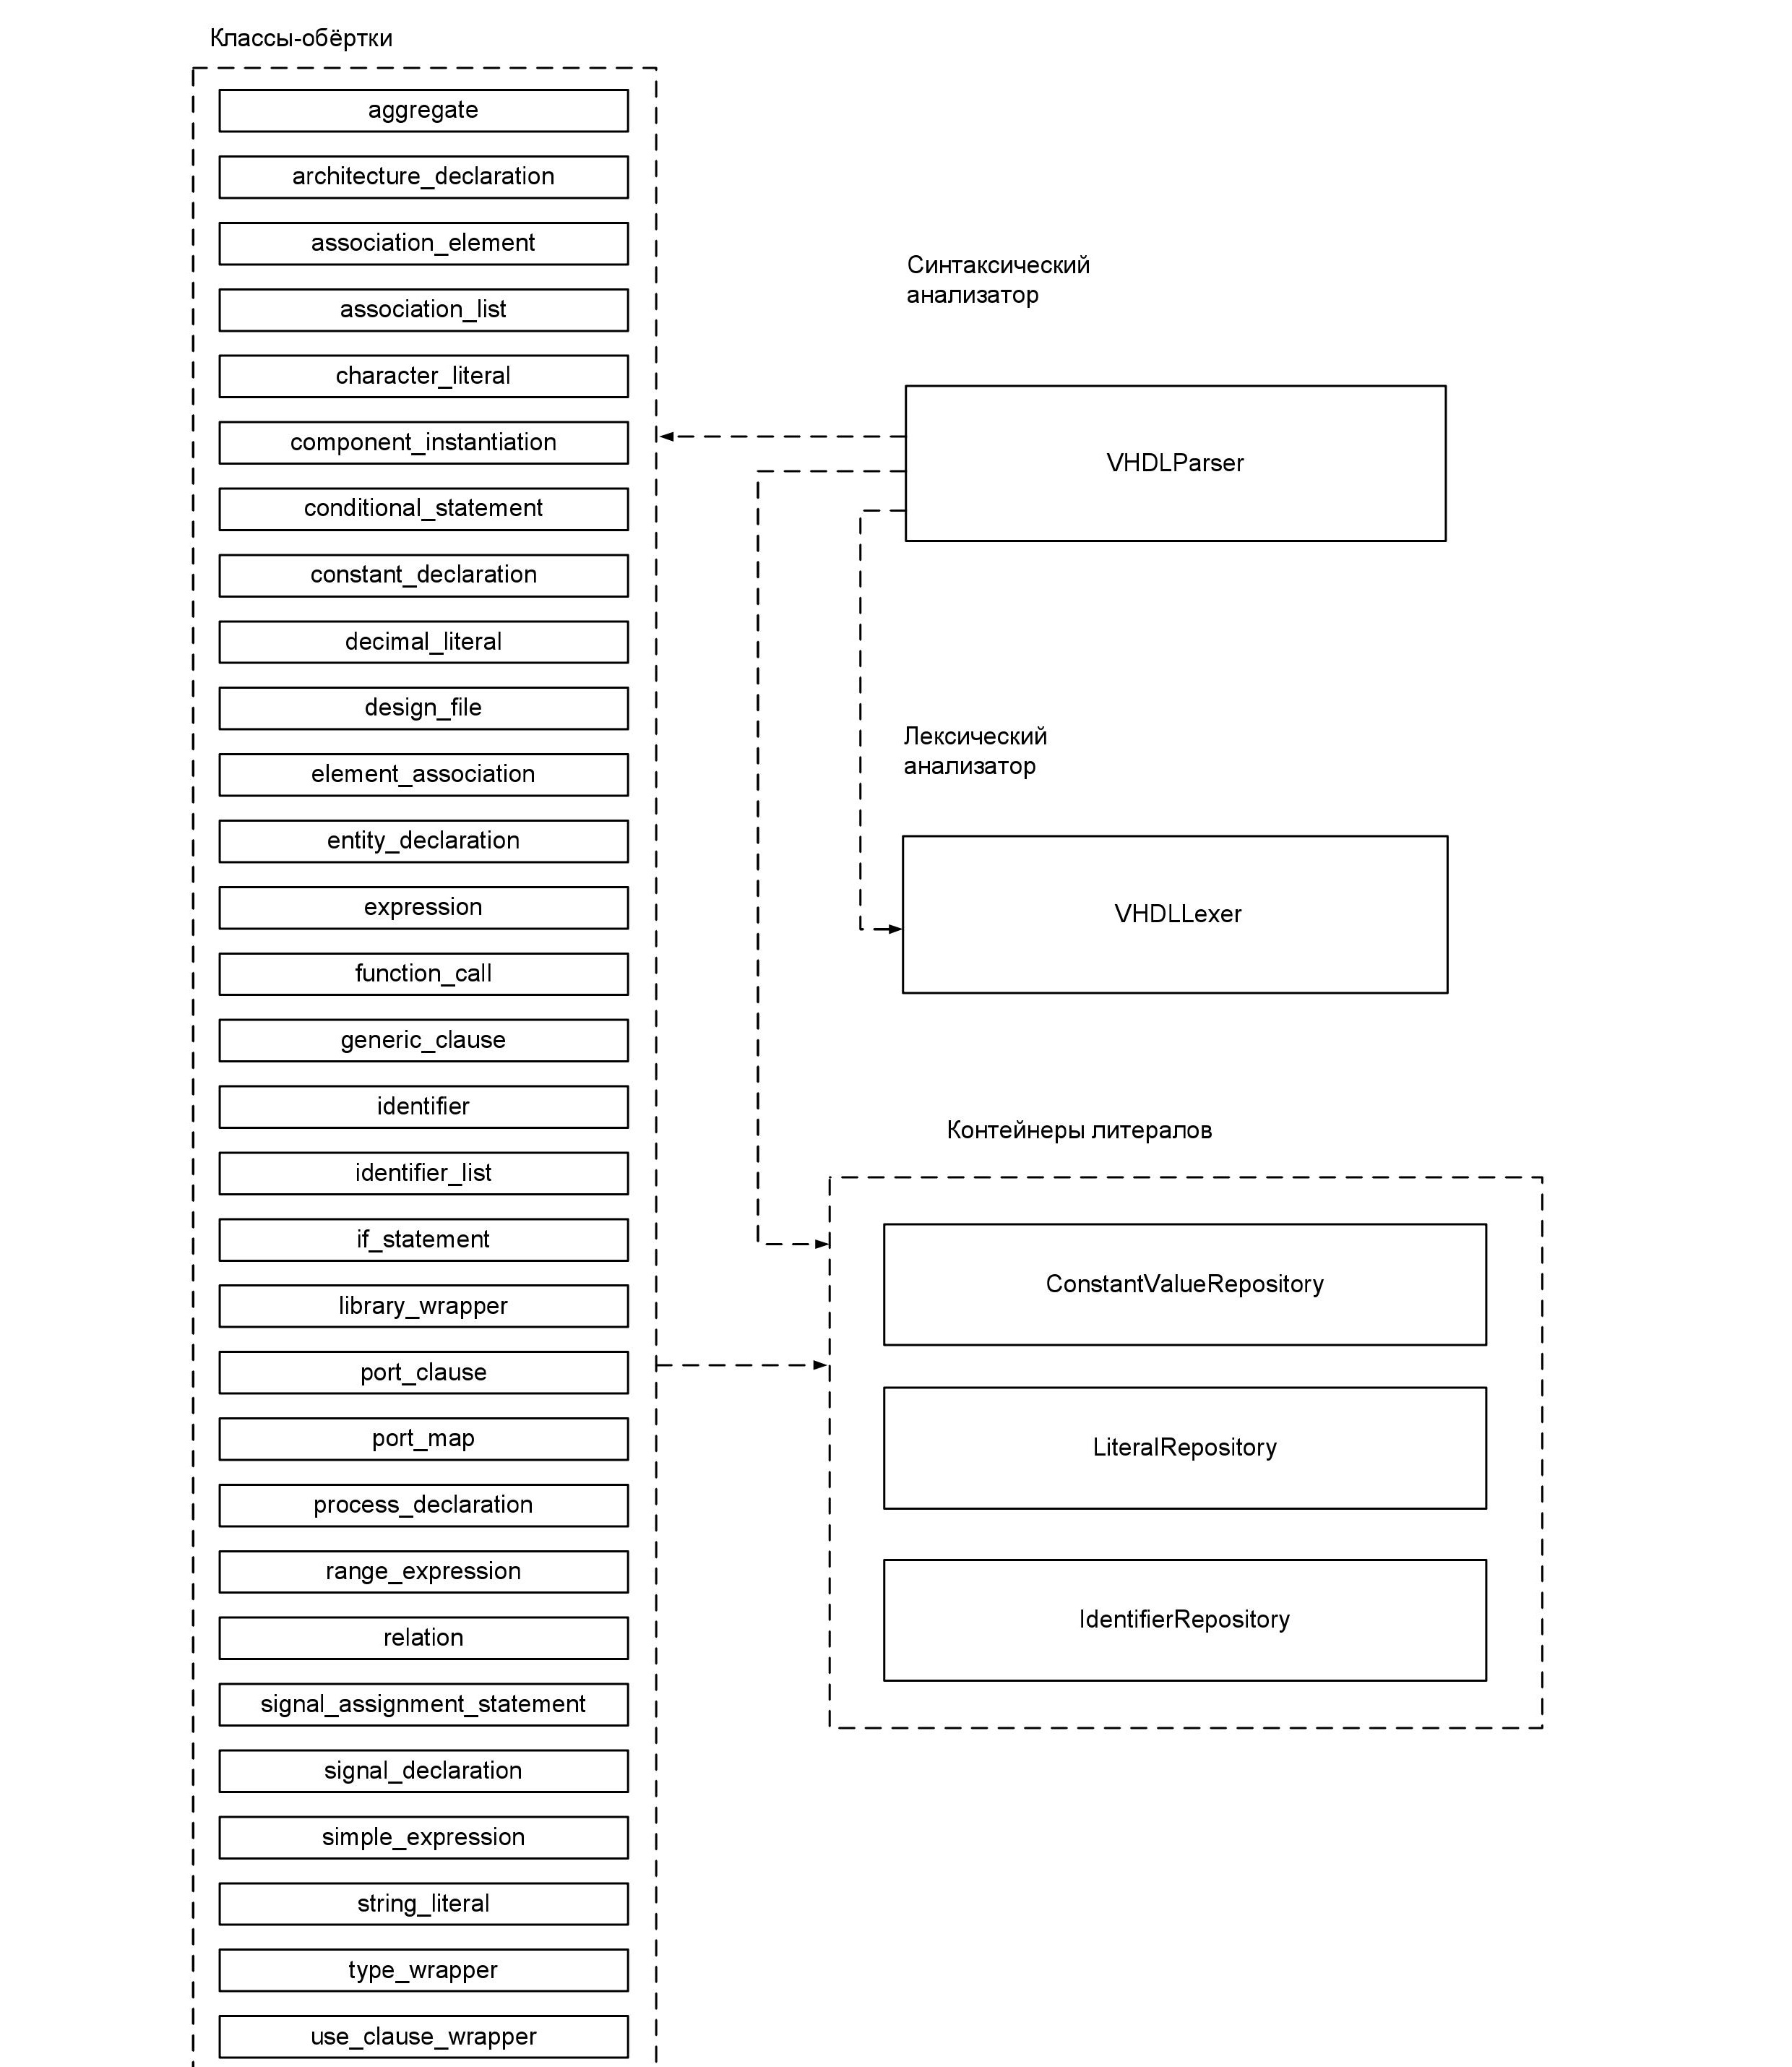
\includegraphics[scale=0.9]{components.jpg}
  \caption{ Диаграмма компонентов программного средства }
  \label{fig:arch_and_mod::components}
\end{figure}
